\documentclass[12pt,a4paper]{ctexart}

\usepackage{geometry}
\usepackage{graphicx}
\usepackage{array}
\usepackage{amsmath}
\usepackage{booktabs}
\usepackage{xeCJK}
\usepackage{tikz}
\usepackage{titlesec}

% 页面设置
\geometry{
    top=2.5cm,
    bottom=2.5cm,
    left=2.8cm,
    right=2.8cm
}

% 定义 section* 格式
\titleformat{\section}
  {\zihao{-3}\heiti\bfseries}
  {}
  {0em}
  {}
\titlespacing*{\section}{0pt}{0.5cm}{0.3cm}  % 左缩进、上间距、下间距


% 取消页码（封面）
\pagestyle{empty}

% 定义等长下划线命令（固定宽度 6.5cm，左对齐）
\newcommand{\infofill}[1]{{\zihao{4}\songti\underline{\makebox[6.5cm][c]{#1}}}}

% 定义内容区块命令
\newcommand{\reportsection}[2]{%
    \noindent{\zihao{-3}\heiti\bfseries #1（#2分）}
    \vspace{0.3cm}
    
    \noindent\rule{\textwidth}{0.4pt}
    \vspace{6cm}
}

% 设置中文字体
\setCJKmainfont{SimSun}  % 宋体，可根据系统改为 Noto Serif CJK SC 等

\begin{document}
% ==================== 封面页 ====================
\begin{titlepage}
    \centering
    \vspace*{1.5cm}
    % 校徽占位（正方形示例图）
    
\includegraphics[width=5cm,height=5cm]{images/image-2026-09-07-14-57-04.png}
    
    \vspace{1.8cm}
    
    % 中山大学
    {\zihao{1}\heiti\bfseries 中山大学}
    
    \vspace{0.9cm}
    
    % 微电子科学与技术学院
    {\zihao{2}\heiti 微电子科学与技术学院}
    
    \vspace{0.9cm}
    
    % 课程名称
    {\zihao{2}\heiti 《集成电路元器件特性表征实验》}
    
    \vspace{0.9cm}
    
    % 实验报告
    {\zihao{1}\heiti\bfseries 实验报告}
    
    \vspace{3cm}
    
    % 信息表格
    

    % 信息表格（无任何框线，无横线，无竖线）
    \begin{tabular}{@{}>{\zihao{4}\heiti}r @{\hspace{1.2em}} l@{}}
        实验主题      & \infofill{半导体材料的霍尔效应测试}        \\[0.8cm]
        姓\quad\quad 名 & \infofill{徐睿琳}   \\[0.8cm]
        学\quad\quad 号 & \infofill{23342107} \\[0.8cm]
        实验日期      & \infofill{\today}   \\[0.8cm]
    \end{tabular}
    
    \vfill
\end{titlepage}

% ==================== 内容页 ====================
\newpage
\pagestyle{plain}
\setcounter{page}{2}

\section*{实验目的（5分）}
\begin{enumerate}
    \item 理解霍尔效应的物理机理：载流子在磁场中受洛伦兹力偏转、霍尔电场建立及电场力与洛伦兹力平衡的动态过程。
    \item 掌握由对称测量法消除热磁效应与不等位电势差等副效应、提取真实霍尔电压 $V_H$ 的方法。
    \item 掌握由 $V_H$ 计算霍尔系数 $R_H$、灵敏度 $K_H$、载流子浓度与霍尔迁移率的方法，并判别半导体导电类型。
    \item 掌握范德堡（van der Pauw）法测量任意形状薄片样品电阻率的原理与操作。
\end{enumerate}

\section*{实验原理（10分）}
\paragraph{1. 霍尔电压与霍尔系数}
如图 4.1 所示，空穴沿 $x$ 方向漂移速度 $v_x$，磁场沿 $z$ 方向，载流子受洛伦兹力
$F_L=qv\times B=qv_xB_z$，沿 $y$ 方向偏转并在样品下表面积累，形成霍尔电场 $E_y$。稳态时电场力与洛伦兹力平衡：
\begin{equation}
    qE_y=qv_xB_z \quad\Rightarrow\quad E_y=v_xB_z=\frac{J_p}{qp}B_z=R_HJ_pB_z .
\end{equation}
由此得霍尔电压
\begin{equation}
    V_H=E_yW=\frac{R_HI_pB_z}{W}=K_HI_pB_z,
    \label{eq:VH}
\end{equation}
其中 $R_H$ 为霍尔系数，$W$ 为样品厚度，$K_H=R_H/W$ 为灵敏度，单位 $\mathrm{mV/(mA\cdot T)}$。

单一载流子导电时 $R_H=1/(qp)$（p 型）、$R_H=-1/(qn)$（n 型），$R_H$ 的符号即指示导电类型。考虑能量无关散射近似下的霍尔散射因子 $\gamma=\langle\tau^2\rangle/\langle\tau\rangle^2$（$\gamma\sim1\!-\!2$），有
\begin{equation}
    R_H=\frac{\gamma}{qp}\ (\text{p型}),\qquad R_H=-\frac{\gamma}{qn}\ (\text{n型}),
\end{equation}
故载流子浓度 $p=\gamma/(qR_H)$（或 $n=-\gamma/(qR_H)$），迁移率
\begin{equation}
    \mu_H=\frac{|R_H|}{\rho}=|R_H|\sigma,
    \qquad \mu_x=\frac{E_y}{E_xB_z}.
\end{equation}
电子、空穴共同参与导电时
\begin{equation}
    R_H=\frac{(p-b^2n)+(\mu_nB)^2(p-n)}{q\left[(p+bn)^2+(\mu_nB)^2(p-n)^2\right]},
    \quad b=\frac{\mu_n}{\mu_p},
\end{equation}
弱场极限 $R_H=(p-b^2n)/[q(p+bn)^2]$，强场极限 $R_H=1/[q(p-n)]$。

\paragraph{2. 副效应与对称测量法}
实测电压中除 $V_H$ 外还叠加不等位电势差、厄廷豪森效应、能斯特效应和里吉--勒迪克效应等热磁副效应。其中仅 $V_H$ 同时随 $I_x$、$B_z$ 反号而改变符号，故依次测量 $(+I,+B)$、$(-I,+B)$、$(-I,-B)$、$(+I,-B)$ 下的 $V_1\!\sim\!V_4$，取
\begin{equation}
    V_H=\frac{V_1-V_2+V_3-V_4}{4},
    \label{eq:sym}
\end{equation}
即可基本抵消上述副效应。

\paragraph{3. 范德堡法测电阻率}
对厚度均匀、无孤立孔洞、四触点足够小的任意形状薄片（图 4.2），由保角映射得
\begin{equation}
    \rho=\frac{\pi W}{\ln 2}\,\frac{R_{12,34}+R_{23,41}}{2}\,F,\qquad
    R_{12,34}=\frac{V_{34}}{I},\ \ R_{23,41}=\frac{V_{41}}{I},
\end{equation}
式中修正因子 $F$ 由比值 $R_r=R_{12,34}/R_{23,41}$ 查图 4.3 确定。结合 $\rho$ 与 $R_H$ 即可求得 $\mu_H=|R_H|/\rho$。

\section*{实验设备和步骤（5分）}
\paragraph{实验设备}
SH500A 霍尔效应实验仪（面板左为励磁电流输入、中为霍尔电压显示、右为霍尔电流输入）、电磁铁线圈、GaAs 霍尔元件（厚度 $W=0.2\ \mathrm{mm}$，最大工作电流 $6\ \mathrm{mA}$，标称灵敏度 $K_H$）。

\paragraph{实验步骤}
\begin{enumerate}
    \item 开机前将励磁电流与霍尔电流旋钮逆时针旋到底，确保无磁场、无电流输出；按面板分区正确连接励磁电流、霍尔电压、霍尔电流三路控制电路。
    \item 记录待测元件标称灵敏度 $K_H$，将元件置于电磁铁气隙中心（磁场均匀区）。
    \item \textbf{固定励磁电流}：$I_M=400\ \mathrm{mA}$（对应 $B=179.7\ \mathrm{mT}$）；霍尔电流由 $1\ \mathrm{mA}$ 增至 $6\ \mathrm{mA}$，步长 $1\ \mathrm{mA}$；每个电流点按式 (\ref{eq:sym}) 的四种极性组合测 $V_1\!\sim\!V_4$ 并求 $V_H$。
    \item \textbf{固定霍尔电流}：$I_H=3\ \mathrm{mA}$；励磁电流由 $300\ \mathrm{mA}$ 增至 $600\ \mathrm{mA}$，步长 $50\ \mathrm{mA}$（对应 $B=134.7\!\sim\!269.2\ \mathrm{mT}$）；同样按四种极性组合测 $V_1\!\sim\!V_4$ 并求 $V_H$。
    \item 按范德堡法接线，依次测 $R_{12,34}$ 与 $R_{23,41}$，由 $R_r$ 查取 $F$ 后计算电阻率 $\rho$。
    \item 测量完毕将两旋钮旋到底后关机，元件归位。
\end{enumerate}

\paragraph{注意事项}
霍尔电流不得超过 $6\ \mathrm{mA}$；元件薄脆，禁止手触与机械挤压；霍尔电流与励磁电流回路不可接错；电磁铁不宜长时间通电，以免线圈发热引起磁场漂移与测量误差。

\section*{实验数据分析（50分）}

\subsection*{1. 霍尔电压的提取}
本实验四种极性组合的读数满足 $|V_1|\approx|V_2|\approx|V_3|\approx|V_4|$，且 $V_3,V_4$ 相对 $V_1,V_2$ 反号，对应实际测量次序为 $(+I_x,+B_z),(-I_x,+B_z),(+I_x,-B_z),(-I_x,-B_z)$。故对称组合取
\begin{equation}
    V_H=\frac{V_1-V_2-V_3+V_4}{4}=\frac{|V_1|+|V_2|+|V_3|+|V_4|}{4},
    \label{eq:VH2}
\end{equation}
该式与手册 $V_H=(V_1-V_2+V_3-V_4)/4$ 在 $V_3,V_4$ 次序互换时等价，均可抵消不等位电势 $V_0$ 及能斯特、里吉--勒迪克等热磁副效应。实测四次读数的偏差均 $<0.8\ \mathrm{mV}$（相对 $<0.4\%$，图 c），表明副效应贡献很小，霍尔电压占绝对主导。

\subsection*{2. 固定励磁电流（$I_M=400\ \mathrm{mA}$，$B=179.7\ \mathrm{mT}$）}
\begin{table}[htbp]\centering\small
\caption{固定磁场下 $V_H$ 随霍尔电流的变化}
\begin{tabular}{ccccccc}\toprule
$I_H$ (mA) & $V_1$ (mV) & $V_2$ (mV) & $V_3$ (mV) & $V_4$ (mV) & $V_H$ (mV) & $K_H$ [mV/(mA$\cdot$T)]\\\midrule
1 &  32.8 &  $-32.9$ &  $-33.1$ &  33.0 &  32.95 & 183.4\\
2 &  65.1 &  $-65.2$ &  $-65.7$ &  65.6 &  65.40 & 182.0\\
3 &  97.5 &  $-97.5$ &  $-98.2$ &  98.2 &  97.85 & 181.5\\
4 & 129.9 & $-129.9$ & $-130.8$ & 130.8 & 130.35 & 181.3\\
5 & 162.3 & $-162.2$ & $-163.4$ & 163.4 & 162.83 & 181.2\\
6 & 194.5 & $-194.4$ & $-195.7$ & 195.8 & 195.10 & 181.0\\\bottomrule
\end{tabular}
\end{table}

\begin{figure}[htbp]
    \centering
    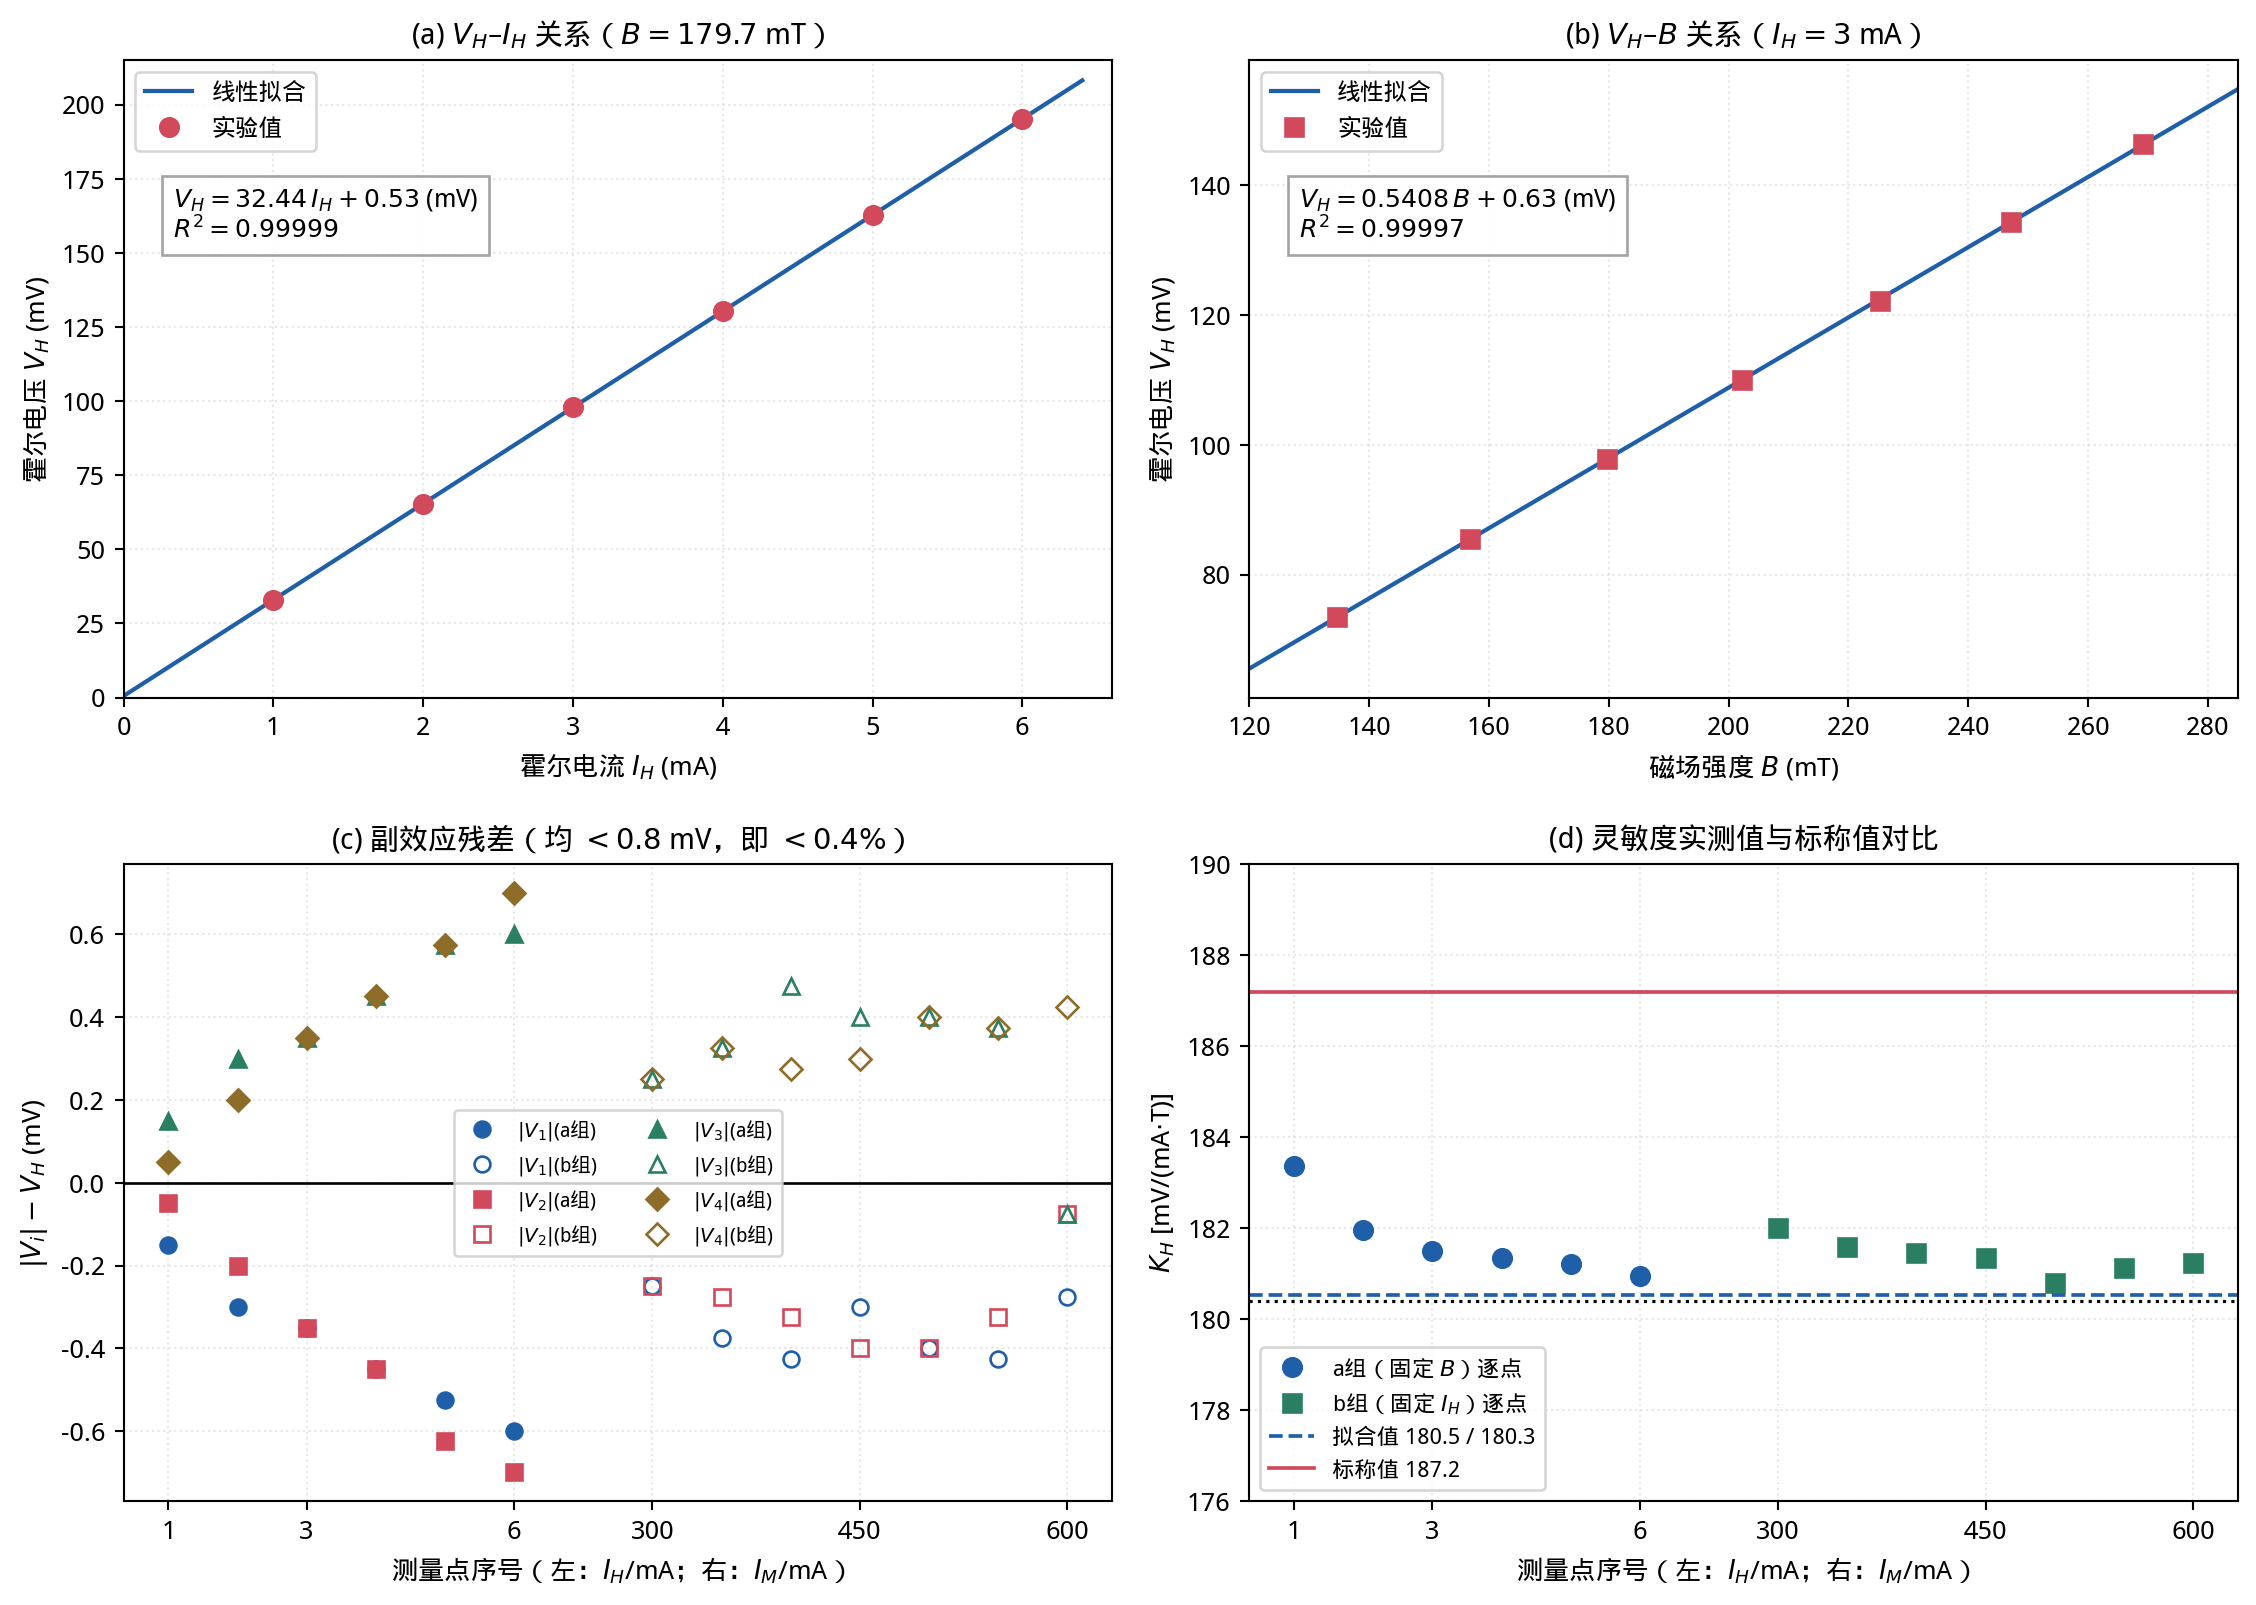
\includegraphics[width=0.75\textwidth]{images/image-2026-10-18-16-05-11.png}
    \caption{固定磁场下 $V_H$ 随霍尔电流 $I_H$ 的变化关系}
    \label{fig:VH-IH}
\end{figure}

$V_H$ 与 $I_H$ 呈良好线性（图 \ref{fig:VH-IH}），最小二乘拟合得
$V_H=(32.44\,I_H+0.53)\ \mathrm{mV}$，$R^2=0.99999$。截距 $0.53\ \mathrm{mV}$ 为仪器零点与残余不等位电势，可忽略。由 $V_H=K_HI_HB$ 得
\begin{equation}
    K_H=\frac{1}{B}\frac{\mathrm{d}V_H}{\mathrm{d}I_H}=\frac{32.44}{0.1797}=180.5\ \mathrm{mV/(mA\cdot T)} .
\end{equation}

\subsection*{3. 固定霍尔电流（$I_H=3\ \mathrm{mA}$）}
\begin{table}[htbp]\centering\small
\caption{固定霍尔电流下 $V_H$ 随磁场的变化}
\begin{tabular}{cccccccc}\toprule
$I_M$ (mA) & $B$ (mT) & $V_1$ & $V_2$ & $V_3$ & $V_4$ & $V_H$ (mV) & $K_H$ [mV/(mA$\cdot$T)]\\\midrule
300 & 134.7 &  73.3 &  $-73.3$ &  $-73.8$ &  73.8 &  73.55 & 182.0\\
350 & 156.9 &  85.1 &  $-85.2$ &  $-85.8$ &  85.8 &  85.48 & 181.6\\
400 & 179.7 &  97.4 &  $-97.5$ &  $-98.3$ &  98.1 &  97.83 & 181.5\\
450 & 202.2 & 109.7 & $-109.6$ & $-110.4$ & 110.3 & 110.00 & 181.3\\
500 & 225.3 & 121.8 & $-121.8$ & $-122.6$ & 122.6 & 122.20 & 180.8\\
550 & 247.2 & 133.9 & $-134.0$ & $-134.7$ & 134.7 & 134.33 & 181.1\\
600 & 269.2 & 146.1 & $-146.3$ & $-146.3$ & 146.8 & 146.38 & 181.3\\\bottomrule
\end{tabular}
\end{table}

拟合得 $V_H=(0.5408\,B+0.63)\ \mathrm{mV}$（$B$ 以 mT 计），$R^2=0.99997$（图 b），故
\begin{equation}
    K_H=\frac{1}{I_H}\frac{\mathrm{d}V_H}{\mathrm{d}B}=\frac{540.8}{3}=180.3\ \mathrm{mV/(mA\cdot T)} .
\end{equation}
两独立数据集所得 $K_H$ 仅相差 $0.2\%$，且在公共点（$3\ \mathrm{mA}$、$179.7\ \mathrm{mT}$）分别给出 $97.85$ 与 $97.83\ \mathrm{mV}$，一致性良好。

\subsection*{4. 霍尔系数与载流子浓度}
由 $K_H=R_H/W$，取 $W=0.2\ \mathrm{mm}$ 及 $\overline{K_H}=180.4\ \mathrm{mV/(mA\cdot T)}$：
\begin{equation}
    R_H=K_HW=180.4\ \frac{\mathrm{V}}{\mathrm{A\cdot T}}\times2.0\times10^{-4}\ \mathrm{m}
        =3.61\times10^{-2}\ \mathrm{m^3/C}=3.61\times10^{4}\ \mathrm{cm^3/C}.
\end{equation}
按记录极性，$(+I_x,+B_z)$ 下 $V_H>0$，故 $R_H>0$，样品为 \textbf{p 型}导电（该结论依赖仪器电压引线极性定义，若接线反接则反号为 n 型）。取霍尔散射因子 $\gamma=1$：
\begin{equation}
    p=\frac{\gamma}{qR_H}=\frac{1}{1.602\times10^{-19}\times3.61\times10^{-2}}
     =1.73\times10^{20}\ \mathrm{m^{-3}}=1.73\times10^{14}\ \mathrm{cm^{-3}} .
\end{equation}
若取声学波散射 $\gamma\approx1.18$，则 $p\approx2.0\times10^{14}\ \mathrm{cm^{-3}}$。霍尔迁移率 $\mu_H=|R_H|/\rho$ 需由范德堡法测得电阻率 $\rho$ 后方可求出，本次未测，故略。

\subsection*{5. 误差分析}
\begin{itemize}
    \item \textbf{与标称值偏差}：实测 $\overline{K_H}=180.4$ 对标称 $187.2\ \mathrm{mV/(mA\cdot T)}$ 偏低 $3.6\%$，两组独立测量一致复现该偏差，属系统误差。可能来源：元件实际厚度与标称 $0.2\ \mathrm{mm}$ 的偏差、标定磁场与实测磁场（线圈发热导致 $B$ 漂移）的差异、灵敏度标签对应温度与实际工作温度不同。
    \item \textbf{副效应}：四次读数离散 $<0.8\ \mathrm{mV}$，对称平均后残余 $<0.4\%$；残余厄廷豪森效应无法由对称法消除，是 $V_H$ 的主要系统误差源。
    \item \textbf{热漂移}：由表 2 逐点 $K_H$ 随 $I_M$ 增大略降（$182.0\!\to\!181.3$），以及表 1 中 $K_H$ 随 $I_H$ 增大略降（$183.4\!\to\!181.0$），提示长时间通电使元件与线圈升温，导致 $B$ 与 $R_H$ 缓慢漂移；实验中应尽量缩短通电时间。
    \item \textbf{其他}：读数有效位仅 $0.1\ \mathrm{mV}$，在 $V_H\!\sim\!33\ \mathrm{mV}$ 处引入约 $0.3\%$ 随机误差；样品未置于气隙严格中心亦会带来磁场误差。
\end{itemize}

\section*{实验结论（20分）}
\begin{enumerate}
    \item \textbf{霍尔效应的线性规律得到验证。} 固定 $B=179.7\ \mathrm{mT}$ 时 $V_H=(32.44I_H+0.53)\ \mathrm{mV}$，$R^2=0.99999$；固定 $I_H=3\ \mathrm{mA}$ 时 $V_H=(0.5408B+0.63)\ \mathrm{mV}$，$R^2=0.99997$。二者共同证明 $V_H\propto I_HB$ 的严格线性关系，且截距均小于 $0.7\ \mathrm{mV}$，说明零点与残余不等位电势可忽略。

    \item \textbf{对称测量法有效抑制了副效应。} 四种极性下 $|V_1|\!\sim\!|V_4|$ 相互偏差 $<0.8\ \mathrm{mV}$（相对 $<0.4\%$），经 $V_H=(V_1-V_2-V_3+V_4)/4$ 处理后，不等位电势、能斯特效应与里吉--勒迪克效应被基本抵消，实测电压中霍尔电压占绝对主导。

    \item \textbf{灵敏度与霍尔系数自洽。} 由两组独立数据分别得 $K_H=180.5$ 与 $180.3\ \mathrm{mV/(mA\cdot T)}$，相对偏差仅 $0.2\%$；取平均 $\overline{K_H}=180.4\ \mathrm{mV/(mA\cdot T)}$，进而
    \[R_H=K_HW=3.61\times10^{-2}\ \mathrm{m^3/C}=3.61\times10^{4}\ \mathrm{cm^3/C}.\]
    两法在公共测量点（$3\ \mathrm{mA}$、$179.7\ \mathrm{mT}$）给出 $97.85$ 与 $97.83\ \mathrm{mV}$，一致性良好，说明结果可靠、可复现。

    \item \textbf{导电类型与载流子浓度。} 按仪器引线极性下 $(+I_x,+B_z)$ 对应 $V_H>0$，即 $R_H>0$，判定样品为 \textbf{p 型}导电（该判定依赖电压引线极性，反接则反号）。取 $\gamma=1$ 得 $p=\gamma/(qR_H)=1.73\times10^{14}\ \mathrm{cm^{-3}}$；若取声学波散射 $\gamma\approx1.18$，则 $p\approx2.0\times10^{14}\ \mathrm{cm^{-3}}$，属轻掺杂外延层量级。

    \item \textbf{与标称值的系统偏差。} 实测 $\overline{K_H}$ 较标称值 $187.2\ \mathrm{mV/(mA\cdot T)}$ 偏低 $3.6\%$，且两组独立测量一致复现，属系统误差而非随机误差。结合逐点灵敏度在大电流、大磁场端单调下降（$182.0\!\to\!181.3$）的现象，可判定主因是电磁铁长时间通电升温导致的磁场衰减，其次为元件实际厚度偏差与标定温度差异；残余厄廷豪森效应无法通过对称法消除，亦是固有误差源。

    \item \textbf{迁移率留待补全。} 霍尔迁移率 $\mu_H=|R_H|/\rho$ 需由范德堡法测得 $\rho$ 后方能给出，本次未完成电阻率测量，故不作数值结论。
\end{enumerate}

\section*{实验启示和拓展（10分）}
\paragraph{方法层面}
\begin{itemize}
    \item \textbf{对称测量是通用的误差分离思想。} 凡目标信号与干扰量对某物理量的奇偶对称性不同，均可用反号组合相消（本实验即利用 $V_H$ 对 $I$、$B$ 均为奇函数，而热磁副效应不全为奇）。该思路可直接迁移到四探针电阻率测量中的电流换向、电桥测量中的交换法。
    \item \textbf{多变量交叉验证优于单次测量。} 本实验以固定 $B$ 扫 $I$、固定 $I$ 扫 $B$ 两种方式独立求 $K_H$，偏差仅 $0.2\%$，才使 $3.6\%$ 的标定偏差被可信地归因于系统误差。单一数据集无法区分随机误差与系统误差。
    \item \textbf{测量行为本身会扰动被测对象。} 大电流注入与电磁铁长时间通电引起的自热，会系统性改变 $B$ 与 $R_H$。实验操作上应遵循「短时通电、读数即断、量程由小到大」的原则，并在高精度测量中引入恒温与温度监测。
\end{itemize}





\end{document}